%http://math.mit.edu/~drew/
%https://math.stackexchange.com/questions/93689/software-for-galois-theory
%SetClassGroupBounds("GRH"); 
%K := QuadraticField(9);
%ClassNumber(K);

%https://en.wikipedia.org/wiki/List_of_triangle_inequalities

\documentclass[12pt, a4paper]{article}
\usepackage[bottom=2cm,top=3cm,left=3cm,right=2cm]{geometry}
\usepackage[utf8]{inputenc}
\usepackage{CJKutf8}
\usepackage{mathtext}
\usepackage{graphicx}
\usepackage{wrapfig}
\usepackage[T1]{fontenc}
\usepackage{blindtext}
\usepackage{tasks}
\usepackage{setspace}
\usepackage{amsmath}
\usepackage{amsfonts}
\usepackage{amssymb}
\usepackage{ wasysym }
\usepackage[portuguese]{babel}
\usepackage[utf8]{inputenc}
\usepackage{mathtext}
\usepackage{graphicx}
\usepackage{wrapfig}
\usepackage[T1]{fontenc}
\usepackage{blindtext}
\usepackage{setspace}
\usepackage{amsmath}
%\usepackage{geometry}
\usepackage{amsthm}
\usepackage{graphics}
%\usepackage{amsfonts}
%\usepackage{lipsum}
\usepackage{amssymb}
\usepackage{CJKutf8} %Pacote para escrever em japonês \begin{CJK}{UTF8}{min} \end{CJK}
\usepackage[portuguese]{babel}
\usepackage{multicol}
% \usepackage{colorspace}
\usepackage{graphicx, color}
\newcommand{\mdc}{{\rm mdc}}
\newcommand{\sen}{{\rm sen}}
\newcommand{\tg}{{\rm tg}}
\newcommand{\cotg}{{\rm cotg}}
\newcommand{\cossec}{{\rm cossec}}
\newcommand{\arctg}{{\rm arctg}}
\newcommand{\arcsen}{{\rm arcsen}}
\newcommand{\pulaquestao}{\newline\newline}
\newcommand{\negrito}[1]{\mbox{\boldmath{$#1$}}} 
\usepackage{pifont}
\newcommand{\heart}{\ensuremath\heartsuit}
\newcommand{\diamonde}{\ensuremath\diamondsuit}
\newtheorem{defi}{Definição}
\newtheorem{propo}{Proposição}
\newtheorem{dem}{Demonstração}
\newtheorem{coro}{Corolário}
\DeclareSymbolFont{extraup}{U}{zavm}{m}{n}
\DeclareMathSymbol{\varheart}{\mathalpha}{extraup}{86}
\DeclareMathSymbol{\vardiamond}{\mathalpha}{extraup}{87}
\setlength{\parindent}{0pt}
\usepackage[framemethod=TikZ]{mdframed}
%\usepackage{lipsum}
\mdfdefinestyle{MyFrame}{%
    linecolor=blue,
    outerlinewidth=2pt,
    roundcorner=20pt,
    innertopmargin=\baselineskip,
    innerbottommargin=\baselineskip,
    innerrightmargin=20pt,
    innerleftmargin=20pt,
    backgroundcolor=white!50!white}
    
%\mdfdefinestyle{Solução}{%
%    linecolor=blue,
%    outerlinewidth=1pt,
%    roundcorner=8pt,
%    innertopmargin=4pt%\baselineskip,
%    innerbottommargin=0pt%\baselineskip,
%    innerrightmargin=20pt,
%    innerleftmargin=20pt,
%    backgroundcolor=white!50!white}
    
    
    \mdfdefinestyle{DAS}{%
    linecolor=blue,
    outerlinewidth=2pt,
    roundcorner=20pt,
    innertopmargin=\baselineskip,
    innerbottommargin=\baselineskip,
    innerrightmargin=20pt,
    innerleftmargin=20pt,
    backgroundcolor=white!50!green}
% \definespotcolor{mygreen}{PANTONE 7716 C}{.83, 0, .00, .51}
% \definespotcolor{tuti}{}{0.6, 0, 1, .508}
\title{PIC - Programa de Iniciação Científica}
\author{Douglas de Araujo Smigly}
\date{}
\begin{document}
\definecolor{Floresta}{rgb}{0.13,0.54,0.13}
\maketitle
\begin{center}
\large\textbf{\textcolor{Floresta}{Ciclo 1 - Encontro 2 - Álgebra}}\\
\end{center}
%\begin{multicols*}{2}
%\setlength{\columnseprule}{0.78pt}
%\raggedcolumns
%\columnbreak
\textcolor{blue}{\bf(1)} (OBMEP 2014) O professor Michel aplicou duas provas a seus alunos e divulgou as notas por meio do gráfico mostrado abaixo. Por exemplo, o aluno A obteve notas 9 e 8 nas provas 1 e 2, respectivamente; já o aluno B obteve notas 3 e 2. Para um aluno ser aprovado, a média aritmética de suas notas deve ser igual a 6 ou maior do que 6. Qual dos gráficos representa a região correspondente às notas de aprovação?
\begin{figure}[!h]
    \centering
    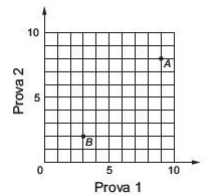
\includegraphics[scale=1.2]{Figuras/1enc2ciclo1.png}
\end{figure}
\begin{tasks}[counter-format={(tsk[a])},label-width=3.6ex, label-format = {\bfseries}, column-sep = {0pt}](3)
\task[\textcolor{Floresta}{$\negrito{(a)} $}] 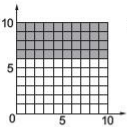
\includegraphics[scale=1.1]{Figuras/2enc2ciclo1.png}
\task[\textcolor{Floresta}{$\negrito{(b)} $}] 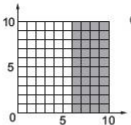
\includegraphics[scale=1.1]{Figuras/3enc2ciclo1.png}
\task[\textcolor{Floresta}{$\negrito{(c)} $}] 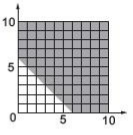
\includegraphics[scale=1.03]{Figuras/4enc2ciclo1.png}
\task[\textcolor{Floresta}{$\negrito{(d)} $}] 
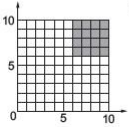
\includegraphics[scale=1.1]{Figuras/5enc2ciclo1.png}
\task[\textcolor{Floresta}{$\negrito{(e)} $}] 
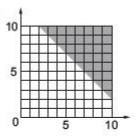
\includegraphics[scale=1.1]{Figuras/6enc2ciclo1.png}
\end{tasks}
\textcolor{blue}{\bf(2)} (OBMEP 2017) Dois carros A e B partem de Quixajuba, ao mesmo tempo, pela estrada que vai para Pirajuba. No gráfico abaixo, a linha contínua e a linha pontilhada representam, respectivamente, a distância de A e B a Quixajuba, ao longo da estrada, em função do tempo.

\begin{figure}[!h]
    \centering
    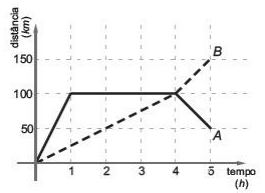
\includegraphics[scale=1.1]{Figuras/7enc2ciclo1.png}
\end{figure}
Qual dos gráficos abaixo representa a distância entre os dois carros, ao longo da estrada, em função do tempo?
\begin{tasks}[counter-format={(tsk[a])},label-width=3.6ex, label-format = {\bfseries}, column-sep = {0pt}](2)
\task[\textcolor{Floresta}{$\negrito{(a)} $}] 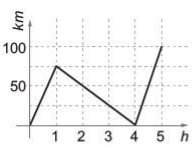
\includegraphics[scale=1.1]{Figuras/8enc2ciclo1.png}
\task[\textcolor{Floresta}{$\negrito{(b)} $}] 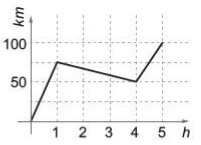
\includegraphics[scale=1.1]{Figuras/9enc2ciclo1.png}
\task[\textcolor{Floresta}{$\negrito{(c)} $}] 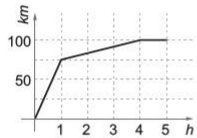
\includegraphics[scale=1.03]{Figuras/10enc2ciclo1.png}
\task[\textcolor{Floresta}{$\negrito{(d)} $}] 
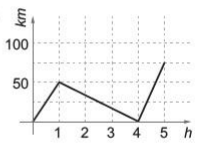
\includegraphics[scale=1.1]{Figuras/11enc2ciclo1.png}
\task[\textcolor{Floresta}{$\negrito{(e)} $}] 
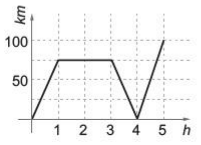
\includegraphics[scale=1.1]{Figuras/12enc2ciclo1.png}
\end{tasks}
\textcolor{blue}{\bf(3)} Em um mesmo dia, Cláudia partiu de Quixajuba para Pirajuba, enquanto Adílson partiu
de Pirajuba para Quixajuba. O gráfico mostra a distância de cada um deles ao respectivo ponto de partida durante todo o trajeto, em função do tempo. A que horas
eles se encontraram na estrada?
\begin{figure}[!h]
    \centering
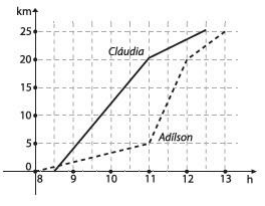
\includegraphics{Figuras/13enc2ciclo1.png}
\end{figure}


\textcolor{blue}{\bf(4)} (OBMEP 2006) Um trabalho de Matemática tem $30$ questões de Aritmética e $50$ de Geometria. Júlia
acertou $70\%$ das questões de Aritmética e $80\%$ do total de questões. Qual o percentual das questões de Geometria que ela acertou?
\newline\newline
\textcolor{blue}{\bf(5)} (OBMEP 2017) Ana e Beto foram os únicos candidatos na eleição para a presidência do grêmio estudantil da escola em que ambos estudam. Nessa eleição, votaram ao todo $1450$ alunos. Durante a apuração, houve um momento em que Ana teve a certeza de que, ao final, ela teria pelo menos a metade dos votos válidos. Naquele momento, os percentuais eram os seguintes:
\begin{itemize}
    \item votos não válidos: $20\%$ dos votos apurados;
    \item votos em Ana: $60\%$ dos votos válidos;
    \item votos em Beto: $40\%$ dos votos válidos.
\end{itemize}
Quantos votos tinham sido apurados até aquele momento?
\newline\newline
\textcolor{blue}{\bf(6)} (OBMEP 2014) Guilherme precisa chegar em $5$ minutos ao aeroporto, que fica a 5 km de sua casa. Se nos $2$ primeiros minutos seu carro andar a uma velocidade média de $90$ km/h, qual é a menor velocidade média que ele terá que desenvolver nos próximos $3$ minutos para não chegar atrasado ao aeroporto?
\newline\newline
\textcolor{blue}{\bf(7)} (OBMEP 2005) No Brasil, usa-se a escala Celsius para medir temperaturas e, em outros países, usa-se a escala Fahrenheit. Para converter uma temperatura da escala Fahrenheit para a Celsius, subtrai-se $32$ do valor da temperatura em graus Fahrenheit e multiplica-se o resultado por $\dfrac{5}{9}.$ Qual dos gráficos representa a relação entre as medidas de uma mesma temperatura em graus \textit{Fahrenheit} (indicados por ºF) e em graus \textit{Celsius}
(indicados por ºC)?
\begin{tasks}[counter-format={(tsk[a])},label-width=3.6ex, label-format = {\bfseries}, column-sep = {0pt}](2)
\task[\textcolor{Floresta}{$\negrito{(a)} $}] 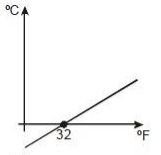
\includegraphics[scale=1.1]{Figuras/14enc2ciclo1.png}
\task[\textcolor{Floresta}{$\negrito{(b)} $}] 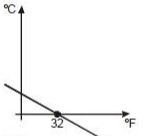
\includegraphics[scale=1.1]{Figuras/15enc2ciclo1.png}
\task[\textcolor{Floresta}{$\negrito{(c)} $}] 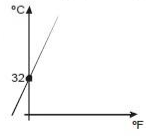
\includegraphics[scale=1.03]{Figuras/16enc2ciclo1.png}
\task[\textcolor{Floresta}{$\negrito{(d)} $}] 
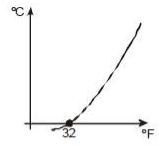
\includegraphics[scale=1.1]{Figuras/17enc2ciclo1.png}
\task[\textcolor{Floresta}{$\negrito{(e)} $}] 
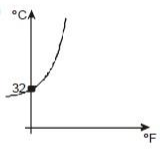
\includegraphics[scale=1.1]{Figuras/18enc2ciclo1.png}
\end{tasks}


\textcolor{blue}{\bf(8)} (OBMEP 2005) Numa certa cidade existem apenas duas empresas de táxi, a Dona Leopoldina e a Dom
Pedro II. A Dona Leopoldina cobra uma taxa fixa de $R\$ 3,00$ mais $R\$ 0,50$ por
quilômetro rodado. Já a Dom Pedro II cobra uma taxa fixa de $R\$ 1,00$ mais $R\$ 0,75$ por quilômetro rodado. Os amigos Bento, Sofia e Helena trabalham nessa cidade e sempre voltam de táxi do trabalho para casa. Para pagar menos, Helena sempre usa os táxis da Dona Leopoldina e, pelo mesmo motivo, Bento só usa os da Dom Pedro II. Sofia usa os táxis das duas empresas, porque paga o mesmo preço em ambas.
\begin{figure}[!h]
    \centering
 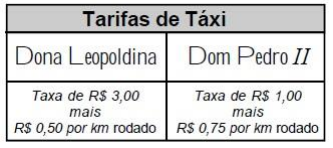
\includegraphics[scale=1.1]{Figuras/19enc2ciclo1.png}
\end{figure}
\begin{tasks}[counter-format={(tsk[a])},label-width=3.6ex, label-format = {\bfseries}, column-sep = {0pt}](2)
\task[\textcolor{Floresta}{$\negrito{(a)} $}] Quanto Sofia paga para ir de táxi do trabalho para casa?
\task[\textcolor{Floresta}{$\negrito{(b)} $}] Qual dos três amigos percorre, de táxi, a menor distância entre seu trabalho e
sua casa?
\end{tasks}

\textcolor{blue}{\bf(9)} Em um grupo de intercâmbio, a razão entre brasileiros e estrangeiros era de $3 : 4.$ Se
cada brasileiro possuía duas canetas e um caderno e cada estrangeiro possuía uma caneta e dois cadernos, calcule a razão entre os números de canetas e cadernos.
\newline\newline
\textcolor{blue}{\bf(10)} Numa loja de automóveis, cada vendedor recebe uma comissão proporcional ao número de carros que vende. Se, em uma semana, o gerente pagou um total de $R\$ 8280,00$ de comissões a quatro funcionários, os quais venderam $3, 6, 7$ e $9$ carros, respectivamente. Quanto ganhou o vendedor que menos carros vendeu?
\newline\newline
\textcolor{blue}{\bf(11)} O custo total, por mês, de um serviço de fotocópias consiste em custo fixo acrescido de um custo variável. O custo variável depende, de forma diretamente proporcional, a quantidade de páginas reproduzidas. Em um mês em que esse serviço fez $50000$ fotocópias, seu custo total foi de $R\$ 21000,00.$ Num outro mês, ao fazer $20000$
cópias, o custo foi de $R\$ 19200,00.$ Qual é o custo por página?
\newline
\newline
\textcolor{blue}{\bf(12)} A fábula da lebre e da tartaruga, do escritor grego Esopo\footnote{Não confundir com Isopor.}, foi recontada utilizando-se o gráfico para descrever os deslocamentos dos animais.
\begin{figure}[!h]
    \centering
 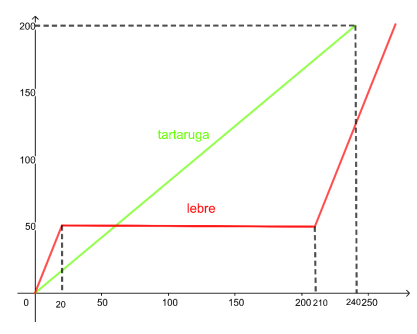
\includegraphics[scale=1.1]{Figuras/20enc2ciclo1.png}
\end{figure}
Para quem não conhece a história, a lebre e a tartaruga apostaram uma corrida. Ao iniciar a corrida, elas partem no mesmo momento e de um mesmo lugar, a lebre começou a correr a uma velocidade constante enquanto a tartaruga foi mais devagar, a uma velocidade constante também. Em um certo momento, a lebre resolve
descansar um pouco e dorme, enquanto a tartaruga continua andando na mesma velocidade. Em um certo momento, quando a tartaruga já tinha ultrapassado a lebre, a lebre acordou e começou a correr rapidamente a uma velocidade constante, tentando alcançar a tartaruga. A tartaruga ganhou a corrida, pois chegou na meta antes que a lebre consiga alcançá-la. A velocidade da lebre após acordar é a mesma de antes de
dormir. O eixo horizontal representa o tempo em minutos e o eixo vertical a distância
em metros. A linha de chegada se encontra a 200 metros de distância da linha de
partida. A linha verde representa o deslocamento da tartaruga e a linha vermelha o
deslocamento da lebre.
\begin{tasks}[counter-format={(tsk[a])},label-width=3.6ex, label-format = {\bfseries}, column-sep = {0pt}](1)
\task[\textcolor{Floresta}{$\negrito{(a)} $}] Determine após quanto tempo, desde o início da corrida, a tartaruga alcançou
a lebre.
\task[\textcolor{Floresta}{$\negrito{(b)} $}] Determine a que distância do ponto de chegada se encontrava a lebre quando
a tartaruga ganhou a corrida.
\end{tasks}
%https://artofproblemsolving.com/community/c6h473647p2651848
\textcolor{blue}{\bf(13) $\varheart$} Sejam $f \colon \mathbb{R} \to \mathbb{R}$ e $g \colon \mathbb{R} \to \mathbb{R}$ duas funções, que satisfazem, para todos $x, y \in \mathbb{R}$
\[
\begin{cases}2f(x+1)-g(x-2)=8x+3 \\f(x+5)+g(x+2)=x+25 \end{cases}
\]
Prove que não existe $x \in \mathbb{R}$ tal que $f(g(x)) = g(f(x)).$
\newline
\newline
\textcolor{blue}{\bf(14) $\varheart$} Seja $f \colon \mathbb{R} \to \mathbb{R}$ uma função tal que
\[
f(x - f(y)) = 1 - x - y, \quad \forall x,y \in \mathbb{R}
\]
Prove que $f$ é uma função afim.
%http://15forum.obmep.org.br/viewtopic.php?f=662&t=10163
\newline
\newline
\textcolor{blue}{\bf(15) $\varheart$} Sejam $m,n $ números naturais positivos distintos, com $m > n.$ Considere $a = m^2 - n^2,$ $b = 2mn$ e $c = m^2 + n^2.$ Mostre que $a,b$ e $c$ são lados de um triângulo retângulo.
\newline
\newline
\textcolor{blue}{\bf(16) $\varheart$} Em um aquário há peixes amarelos e vermelhos.
\begin{tasks}[counter-format={(tsk[a])},label-width=3.6ex, label-format = {\bfseries}, column-sep = {0pt}](1)
\task[\textcolor{Floresta}{$\negrito{(a)} $}] Considere que $90\%$ são amarelos e $10\%$ são vermelhos. Uma misteriosa doença matou muitos peixes amarelos, mas nenhum vermelho. Depois que a doença foi controlada, verificou-se que no aquário $75\%$ dos peixes vivos eram amarelos. Aproximadamente, que porcentagem dos peixes amarelos morreram?
\task[\textcolor{Floresta}{$\negrito{(b)} $}] Vamos generalizar o item anterior. Sejam $0 < p,q < 1.$ Suponha que a porcentagem de peixes amarelos no aquário é $p,$ e que a doença misteriosa matou apenas peixes amarelos, e que depois que a doença foi controlada, a porcentagem de peixes vivos que eram amarelos era $q.$ Mostre que a porcentagem de peixes amarelos que morreram é dada por
\[
1 - \dfrac{q(1-p)}{p(1-q)}.
\]
\end{tasks}
\textcolor{blue}{\bf(17) $\varheart$} Seja $f: \mathbb{R} \rightarrow \mathbb{R}$ uma função. Prove que:
\begin{tasks}[counter-format={(tsk[a])},label-width=3.6ex, label-format = {\bfseries}, column-sep = {0pt}](1)
\task[\textcolor{Floresta}{$\negrito{(a)} $}] $f$ é uma função afim se, e somente se, a taxa de variação $\dfrac{f(x + h) - f(x)}{h}$ é constante, para quaisquer,$x, h \in \mathbb{R},$ com $h > 0.$ Neste caso, temos $f(x) = ax + b,$ onde $a$ é o valor constante da taxa de variação e $b = f(0).$
\task[\textcolor{Floresta}{$\negrito{(b)} $}] Uma função afim dada por $f(x) = ax + b$ é crescente se, e somente se, $a > 0$, e é decrescente se, e somente se, $a < 0.$ Ou seja, toda função afim é monótona.
\end{tasks}
\textcolor{blue}{\bf(18) $\varheart$} Suponha que exista uma função $f \colon \mathbb{N} \to \mathbb{N}$ tal que 
\[
f(2n + f(n)) = n.
\]
Prove que $f$ é sobrejetora.
Exercícios marcados com $\varheart$ são extras.
\end{document}
SetClassGroupBounds("GRH"); 
K := QuadraticField(9);
ClassNumber(K);
Q := PolynomialRing(GF(2), 2);
Q;
K := QuadraticField();
G := GaloisGroup(K);
G;
\begin{CJK}{UTF8}{min}
露の世は 露の世ながら さりながら当時では老人と呼べる50歳代半ばでようやく授かったわが子への愛とその突然死を伝えた「露の世」のくだりは、その日記体句文集「おらが春」のクライマックスとなっています。

5月には数え二歳の誕生を迎えて詠んだ句に、
「這へ笑へ二つになるぞけさからは」と喜びを謳歌したばかり。

それが、翌6月にはもはや草葉の陰へと、その露の朝日に立ちどころに消えるごとく、儚くも身罷ってしまったとは。

人の世は朝露の如く無常なのだと、悔みを述べ慰問するあの人、この人。さは「さりながら」…それは確かにそうなのだけれども。
いかに「あきらめ顔しても、思い切りがたきは、恩愛のきづな也けり。」と、わが心中は耐えきれず切々と泣き崩れるばかり。わが子「さと」女を思う「大切」はやがて「あなた任せ」の境地へと通じていくものでしょう。
\end{CJK}